\documentclass[a4paper, 12pt]{article}

\usepackage[T2A]{fontenc}
\usepackage[utf8]{inputenc}
\usepackage[russian]{babel}
\usepackage{geometry}
\usepackage{setspace}
\usepackage{hyperref}
\usepackage{listings}
\usepackage{graphicx}
\usepackage{indentfirst}
\usepackage{titlesec}
\usepackage{pgfplots}
\usepackage{pgfplotstable}

\pgfplotsset{width=12cm, compat=1.18}
\newgeometry{left=1.5 cm, right=1.5cm, top=1.5cm, bottom=1.5cm}

\begin{document}


% ---------------------------------- Титульник ----------------------------------
\hypersetup{pageanchor=false}
\begin{titlepage}
 \begin{center}
  \vspace*{1cm}

  \Huge
  \textbf{Лабораторная работа №3}

  \vspace{0.5cm}
  \LARGE
  ``Реализация алгоритма с использованием технологии OpenMP''

  \vspace{1.5cm}
  Выполнил студент группы Б20-505\\
  \textbf{Сорочан Илья}

  \vfill

  \Large
  Московский Инженерно-Физический Интститут\\
  Москва 2023

 \end{center}
\end{titlepage}


% ---------------------------------- Рабочая среда ----------------------------------

\section{Рабочая среда}

Технические характеристики (вывод \textit{inxi}):
\begin{verbatim}
CPU: 6-core AMD Ryzen 5 4500U with Radeon Graphics (-MCP-)
speed/min/max: 1396/1400/2375 MHz Kernel: 5.15.85-1-MANJARO x86_64 Up: 46m
Mem: 2689.5/7303.9 MiB (36.8%) Storage: 238.47 GiB (12.6% used) Procs: 238
Shell: Zsh inxi: 3.3.24
\end{verbatim}

Используемый компилятор:
\begin{verbatim}
gcc (GCC) 12.2.0
\end{verbatim}

Согласно \href{https://www.openmp.org/resources/openmp-compilers-tools/}{официальной документации} даная версия компилятора поддерживает \textit{OpenMP 5.0}


% ---------------------------------- Сортировка Шелла ----------------------------------

\section{Реализация алгоритма в одном потоке}

При сортировке Шелла сначала сравниваются и сортируются между собой значения, стоящие один от другого на некотором расстоянии $d$. После этого процедура повторяется для некоторых меньших значений $d$, а завершается сортировка Шелла упорядочиванием элементов при $d = 1$ (то есть обычной сортировкой вставками). Эффективность сортировки Шелла в определённых случаях обеспечивается тем, что элементы «быстрее» встают на свои места (в простых методах сортировки, например, пузырьковой, каждая перестановка двух элементов уменьшает количество инверсий в списке максимум на 1, а при сортировке Шелла это число может быть больше).

Для определённости будет рассматриваться классический вариант, когда изначально $d = \frac{count}{2}$ и уменьшается по закону $d_{i+1} = \frac{d_{i}}{2}$, пока не достигнет $1$. Здесь $count$ обозначает длинну сортируемого массива.

Тогда в худшем случае сортировка займет $O(count^2)$.

Блок схема сортировки Шелла:\\
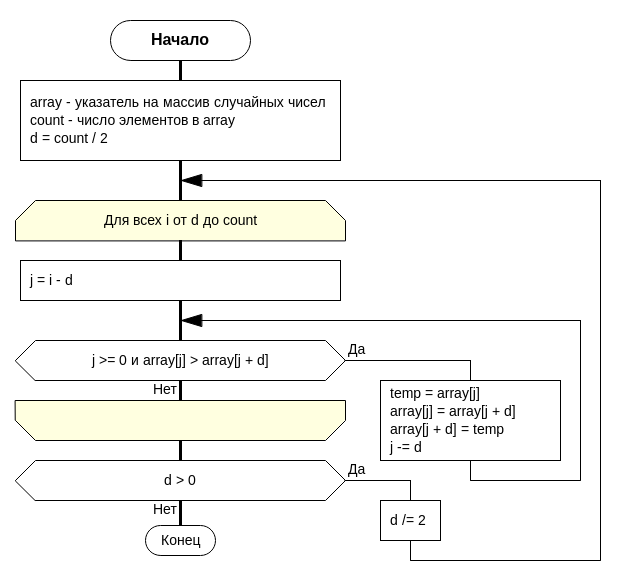
\includegraphics[scale=0.6]{res/original.png}


% ---------------------------------- Параллелизация ----------------------------------

\section{Параллелизация}

Как и в предыдущих работах, в первую очередь параллелизируется цикл.

В первую очередь задаем число потоков и общие переменные через \textit{omp parallel}. Однозначно общими должны быть массив и его длинна.

Так как внутренний цикл по i по сути затрагивает только $d$-e элементы отностительно $i$-го, то его можно параллелизировать:

\begin{lstlisting}[language=C, basicstyle=\scriptsize]
 #pragma omp parallel num_threads(THREADS) shared(array, count) default(none)
    for (int d = count / 2; d > 0; d /= 2) {
        const int cd = d;
        #pragma omp for
        for (int i = cd; i < count; ++i) {
            for (int j = i - cd; j >= 0 && array[j] > array[j + cd]; j -= cd) {
                int temp = array[j];
                array[j] = array[j + cd];
                array[j + cd] = temp;
            }
        }
    }
\end{lstlisting}

Здесь так же видно, что $d$ вынесена в константу $cd$. Это сделано для того, что бы \textit{OpenMP} не принял меры предосторожности в цикле по $i$. Он может это сделать так как $d$ меняется во внешнем цикле, но он не знает меняется ли во внутреннем.


% ---------------------------------- Графики ----------------------------------

\section{Экспериментальные данные}

Во всех измерениях бралось 10 запусков на поток.

В этот раз я решил увеличить количество элементов и худшее время уже доходит до секунды. Однако, как видно ниже на результатах это сказалось не сильно.

\vspace{0.3cm}

\begin{tikzpicture}
 \begin{axis}[
    xlabel={Число потоков},
    ylabel={Время (мс)},
    legend pos=north east,
  ]
  \addplot table [x=Threads, y=Worst (ms), col sep=comma] {data/data.csv};
  \addplot table [x=Threads, y=Best (ms), col sep=comma] {data/data.csv};
  \addplot table [x=Threads, y=Average (ms), col sep=comma] {data/data.csv};
  \legend{Худшее время, Лучшее время, Среднее время}
 \end{axis}
\end{tikzpicture}

\vspace{0.5cm}

Из графика видно, что в среднем многопоточная программа работает медленнее, что на мой взгляд странно. В этой лабораторной, в отличие от предыдущих, алгоритм куда сложнее. Видимо этого недостаточно.

Ну и как уже упоминалось в прошлой работе -- оптимизации компилятора. Ниже приведена таблица для компиляции с \textit{-O3}:

\vspace{0.3cm}

\begin{tikzpicture}
 \begin{axis}[
    xlabel={Число потоков},
    ylabel={Среднее время (мс)},
    legend pos=north east,
  ]
  \addplot table [x=Threads, y=Worst (ms), col sep=comma] {data/optimized.csv};
  \addplot table [x=Threads, y=Best (ms), col sep=comma] {data/optimized.csv};
  \addplot table [x=Threads, y=Average (ms), col sep=comma] {data/optimized.csv};
  \legend{Худшее время, Лучшее время, Среднее время}
 \end{axis}
\end{tikzpicture}

\vspace{0.3cm}

Прекрасно видно, что однопоточная программа лидирует с большим отрывом и причиной этому -- оптимизации компилятора.

Стоит заметить, что многопотчные сборки так же получили прирост и общая тенденция неизменна. Я полагаю, что \textit{OpenMP} мешает компилятору как-то все сильно оптимизировать:

\vspace{0.3cm}

\begin{tikzpicture}
 \begin{axis}[
    xlabel={Число потоков},
    ylabel={Среднее время (мс)},
    legend pos=north east,
  ]
  \addplot table [x=Threads, y=Average (ms), col sep=comma] {data/data.csv};
  \addplot table [x=Threads, y=Average (ms), col sep=comma] {data/optimized.csv};
  \legend{Без \textit{-O3}, C \textit{-O3}}
 \end{axis}
\end{tikzpicture}

\vspace{0.3cm}

Рассмотрим так же прирост, даваймый каждым числом процессоров относительно первого (берем среднее время):

\begin{tikzpicture}
 \begin{axis}[
    xlabel={Число потоков},
    ylabel={Прирост (\%)},
    ybar interval=0.7,
  ]
  \addplot table [x index=0, y index=1, col sep=comma] {data/compare.csv};
 \end{axis}
\end{tikzpicture}

Интересно, что в отличие от предыдущих исследований здесь лидируют сборки с 2 и 3 потоками.

% ---------------------------------- Заключение ----------------------------------

\section{Заключение}
В данной работе было исследовано ускорение, получаемое при использовании многопоточности в сортировке Шелла. Была усовершенствована предоставленная программа и написан специальный скрипт, собирающие данные о нескольких запусках этой программы в один файл, попутно её перекомпилируя.

В ходе работы было выяснено, что в данной задаче применение многопоточности лишь замедлит программу. С уверенностью можно сказать, что частью причины таких результатов являются оптимизации, производимые компилятором.

С другой стороны следует отметить, что для настолько тривиальной задачи применять многопоточность нет смысла. В Экспериментальном массиве сортировалось миллион элементов и даже так, сборка без потоков и со всеми оптимизациями занимала сотые доли миллисекунд.

\appendix

\titleformat{\section}[display]
  {\normalfont\Large\bfseries}
  {\centering Приложение\ \thesection\\}
  {0pt}{\Large\centering}
\renewcommand{\thesection}{\Asbuk{section}}

\section{Использованные программные коды}


Код без многопоточности:
\lstinputlisting[language=C, basicstyle=\small]{src/main.c}
\vspace{0.5cm}

Код с многопоточностью:
\lstinputlisting[language=C, basicstyle=\scriptsize]{src/threaded.c}
\vspace{0.5cm}

Для сборки данных использовался следующий скрипт:
\lstinputlisting[language=Python, basicstyle=\tiny]{src/main.py}
\vspace{0.5cm}

Для вычисления относительного прироста производительности использовался следующий скрипт:
\lstinputlisting[language=Python, basicstyle=\footnotesize]{src/compare.py}
\vspace{0.5cm}

\section{Таблицы с теоритическими и практическими результатами}

Таблица без оптимизаций:

\vspace{0.3cm}

\pgfplotstabletypeset[
 col sep=comma,
 columns={Threads,Worst (ms),Best (ms),Average (ms)},
]{data/data.csv}

\vspace{0.5cm}

Таблица с оптимизациями:

\vspace{0.3cm}

\pgfplotstabletypeset[
 col sep=comma,
 columns={Threads,Worst (ms),Best (ms),Average (ms)},
]{data/optimized.csv}

\vspace{0.5cm}

Таблица сравнений:

\vspace{0.3cm}

\pgfplotstabletypeset[
 col sep=comma,
 columns={Threads,Efficiency},
]{data/compare.csv}


\end{document}
